\documentclass{article}
\usepackage{amsmath}
\usepackage{amssymb}
\usepackage{tabularx}
\usepackage{amsmath}
\usepackage{graphicx}
\graphicspath{ {./diagrams/} }

\begin{document}
\setlength{\parindent}{0in}

\begin {center}
\large Thesis
\end{center}

\section{State of the art}
\subsection{Similar Games}
\subsubsection{Keep Talking and Nobody Explodes}
The game consists in defusing a ticking bomb by solving puzzles attatched to it. It's a two player game, one player is the defuser and the other has a bomb-defusal manual. The players have to exchange the puzzle descriptions and solutions. 
\subsubsection{Unrailed}
The game consists in constructing a railway in front of a moving train. If the trains runs out of track, the game is over. In order to construct rails, the players have to chop trees, mine stone and combine materials in a specialized train cart. It's a 2 to 4 player game. The players  usually talk to split tasks among themselves and get time-sensitive tasks done quickly.
\subsubsection{Among Us}
The game is a mafia game between two teams, impostors and crewmates. A team wins if the other team is dead, crewmates also win when they complete all tasks. Impostors may kill crewmates. If a crewmate finds a corpse, he may call a vote. The player who has to most votes is killed. The players have to discuss who to kill in a limited time.
\subsection{Asymmetric Multiplayer}
A game has asymmetrical multiplayer when the players play the game differently. There are multiple levels of asymmetry: from a slight imbalance in the mechanics to a completely separate set of rules. Keep Talking and Nobody Explodes is the most asymmetrical game in the cited games: a player just has a manual. The other two games have a lesser degree of imbalance: in Unrailed the roles and tasks can be exchanged during the games and in amongus every player is controlling a character and interacting in the game's map.

\clearpage

\section{Applications}
\subsection{Applicable scenarios}
Firefighters in airports, cave exploration.
\subsection{Efficent communication skill development}
The game is focused in training the communication skills of the player. The games puts the player under time pressure and requires a significant amount of information to be exchanged quickly. The game also forces a half duplex communication protocol emulating a radio, such that only one player may speak at a time.
\subsection{Feedback on skill improvements}

\clearpage

\section{Technology used}
\subsection{Input and Devices}
The game will be played using mouse and keyboard. The courier players will only have to use the keyboard.
\subsection{Kinematic Bycicle Model}
\subsection{UDP with optional retransmission}
\subsection{Model View Controller}
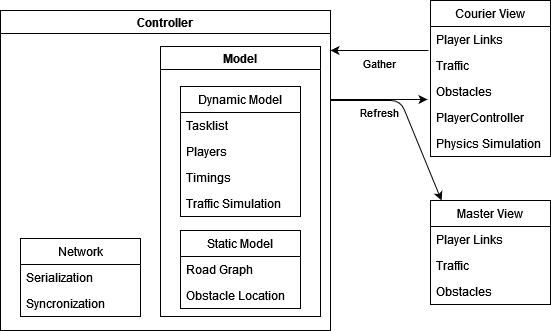
\includegraphics[width=\textwidth]{game architecture}
\subsection{Unity}
\subsection{Optimizations Techniques}

\clearpage

\section{Design}
\subsection{Game Design}
The game is set in a city, with gridstyle roads.
There are up to 2 couriers, which have to fulfil a list of delivery orders.
There is a master player who has a map, which shows the courier's positions and the streets status. The master has the order list, the couriers do not.
The orders consist of a pickup site and dropoff site.
The streets are blocked by many obstacles:
\begin{itemize}
  \item variable level of traffic makes the street difficult to navigate
  \item a drawbridge over a river or a rail
  \item a rail passage getting closed when a train crosses
\end{itemize}
The master has to plan the route during the time and relay the path to each courier in the broadcast channel.
The master's map is outfitted with a shortest path algorithm to ease finding a fast route.
The couriers drive following the Master path, they only see the pickup points and if they have picked up an item, the corrisponding dropoff point.
\subsection{Traffic simulation}
The traffic simulation can be tuned to different levels of complexity.
\subsubsection{Static}
The streets are filled with a random amount of immoble cars.
\subsubsection{Dynamic}
Every street has a traffic level associated to it. The traffic levels oscillate smoothly, but randomly over time. The cars are immoble, but when they are not seen by any players, the amount of cars in a street is adjusted to be proportional to the traffic level of the street.
\subsubsection{Agent Based}
The cars are agents that move thorugh a graph representation of the streets. The cars roam through the city by turning randomly at intersections. The cars respect traffic lights and obstacles on the streets, so that traffic jams happen dynamically.
\subsection{Variations}
\subsubsection{Events}
Throughout the city there are billboards and signs that contain the time and place an event will happen. The event (for example a parade, a festival, the street market, a strike) generates a lot of foot traffic and car traffic in a particular place. The master has no information about these events, so he has to rely on the couriers who will see the billboards and relay the information.
\subsubsection{Delivery Timers}
The delivery orders may have up to three additional timers: a time after which the order is failed if it's not picked up, a delivery time constraint and a time after which the order is failed if not completed.
\subsection{Syncronization model}
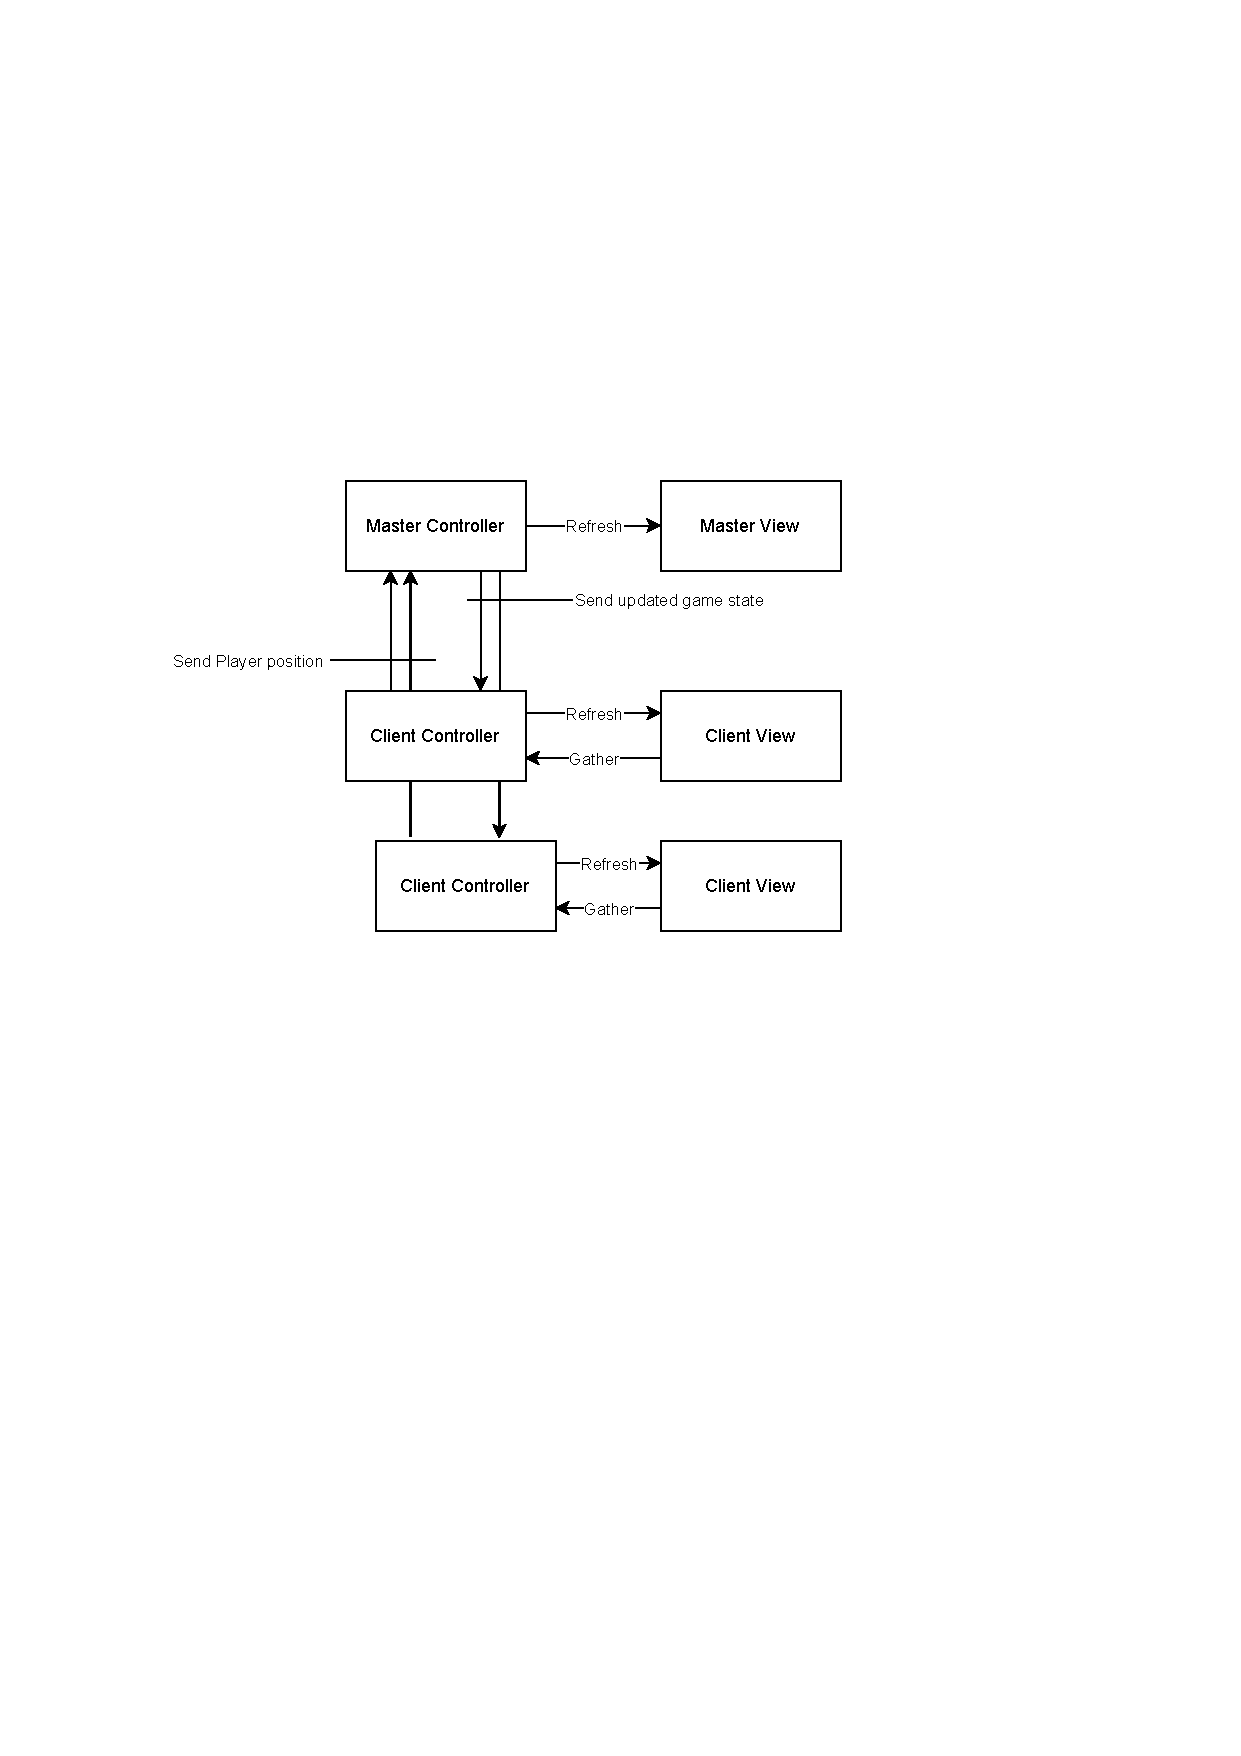
\includegraphics[width=\textwidth]{net architecture}

\clearpage

\section{Testing}
\subsection{Unit Testing and TDD}
\subsection{Integration Testing}

\end{document}